\chapter{Evaluation}\label{ch:eval}

Correctness, performance, and ease of use are three important dimensions along which this project was evaluated.

This section outlines the steps taken to test these, and the results obtained.
The data collection and processing methodology is touched upon.
Known limitations in the implementation are also mentioned.


\section{Overall results}\label{sec:eval:overall}

The final project weighed in at approximately 3,200 lines of Elixir code (excluding comments, blank lines and tests).
Approximately 12,000 lines of code were written over the lifetime of the project, illustrating the volatility of the codebase due to evolving requirements.



\section{Correctness testing}\label{sec:eval:correctness}

Unit tests were written for individual modules using the ExUnit library <ref>.

\section{Known limitations}\label{sec:eval:limitations}

This project implements only a core of features from the Beam Model.
There are many known limitations and missing features.
Most of these are due to time constraints in the project, compounded with changing assumptions driving some less-than-optimal decisions earlier in the process.

branching pipelines---need dispatcher\\
side inputs\\
type-checking\\
sessions / unaligned windows in general\\
source/sink API\\


\todo{include capability matrices? Maybe construct one for this implementation? (https://beam.apache.org/documentation/runners/capability-matrix/)}

\section{Approach to empirical evaluation}\label{sec:eval:approach}

\subsection{Test environment}\label{sec:eval:approach:environment}

Efforts were made to collect data in similar environments in order to reduce the potential for uncontrolled variation.

All tests were conducted on a single machine, a MacBook Pro (15-inch, Late 2016) with a 2.9GHz Intel Core i7 CPU and 16GB of 2133 MHz RAM running macOS 10.12.4.
Runtimes used were Elixir 1.4.2 on OTP 19 and the Oracle JRE v1.8.0\_66-b17.

Prior to conducting the tests, all non-essential background processes and applications were terminated.
Tests were initiated using scripts in order to replicate multiple instances of the tests accurately.

Some of the evaluation (\cref{sec:eval:approach:twitter}) depended on an external stream of data from Twitter.
Due to time constraints and the complexity of the API, it was not feasible to set up a mock server to serve identical data at each execution.
However, informal observation of the data stream show it has a relatively consistent throughput, minimising time-of-execution effects.
Additionally, the tests were executed multiple times throughout the day and the data averaged and aggregated to arrive at the final results, minimising the effects of any variation.

\subsection{Data collection and processing methodologies}\label{sec:eval:approach:collection}

A custom test runner was developed in Elixir for the purpose of scheduling and running tests.
It could be configured with the tests to be run for both the Java and Elixir implementations.
Each test was executed via a new system process with configuration passed as command-line arguments.
A new VM instance was created each time for both Elixir and Java tests to maintain consistency and accuracy.

The test runner measured the CPU and memory usage of the spawned process using the \verb|ps| program.
Other measurements, such as latency, were taken directly in the executing test and saved to the appropriate directory (as passed by the runner through the command line).

The data were then processed, analysed and plotted using MATLAB.
Sources for both the test runner and the MATLAB scripts used can be found in \cref{apx:twitter-code}.

\section{The Twitter example}\label{sec:eval:approach:twitter}

Twitter is a popular social network focused on posting short messages, or \emph{statuses}.
Statuses tend to include \emph{hashtags}, words or short phrases preceded by the \# character.
Hashtags rely on many users using the exact hashtag text in their tweets.
The hashtag can then be used to aggregate and list all of these tweets, perhaps on a particular topic.

It is reasonable, therefore, that an autocomplete functionality may be useful for hashtag entry, to suggest popular hashtags and discourage misspellings.
This real-world scenario formed the basis of this evaluation exercise.

Twitter's free streaming API \cite{TwitterStreamingAPI} was used to receive a stream of English-language tweets on particular topics.
The terms `tracked' to select topics were \texttt{["tech", "technology", "Apple", "Google", "Twitter", "Facebook", "Microsoft", "iPhone", "Mac", "Android", "computers", "CompSci", "science"]}.

The tweets were windowed using sliding windows and then processed further.
Hashtags present were counted per-window.
They were then expanded into all possible prefixes, retaining counts.
Finally, a list of the top three hashtag suggestions for each prefix was produced.
This data could be fed into an autocompletion API, but for the purposes of this exercise was simply printed to console.
\Cref{fig:eval:twitter-pipeline-dag} illustrates the resultant Pipeline.

\begin{figure}
	\centering
	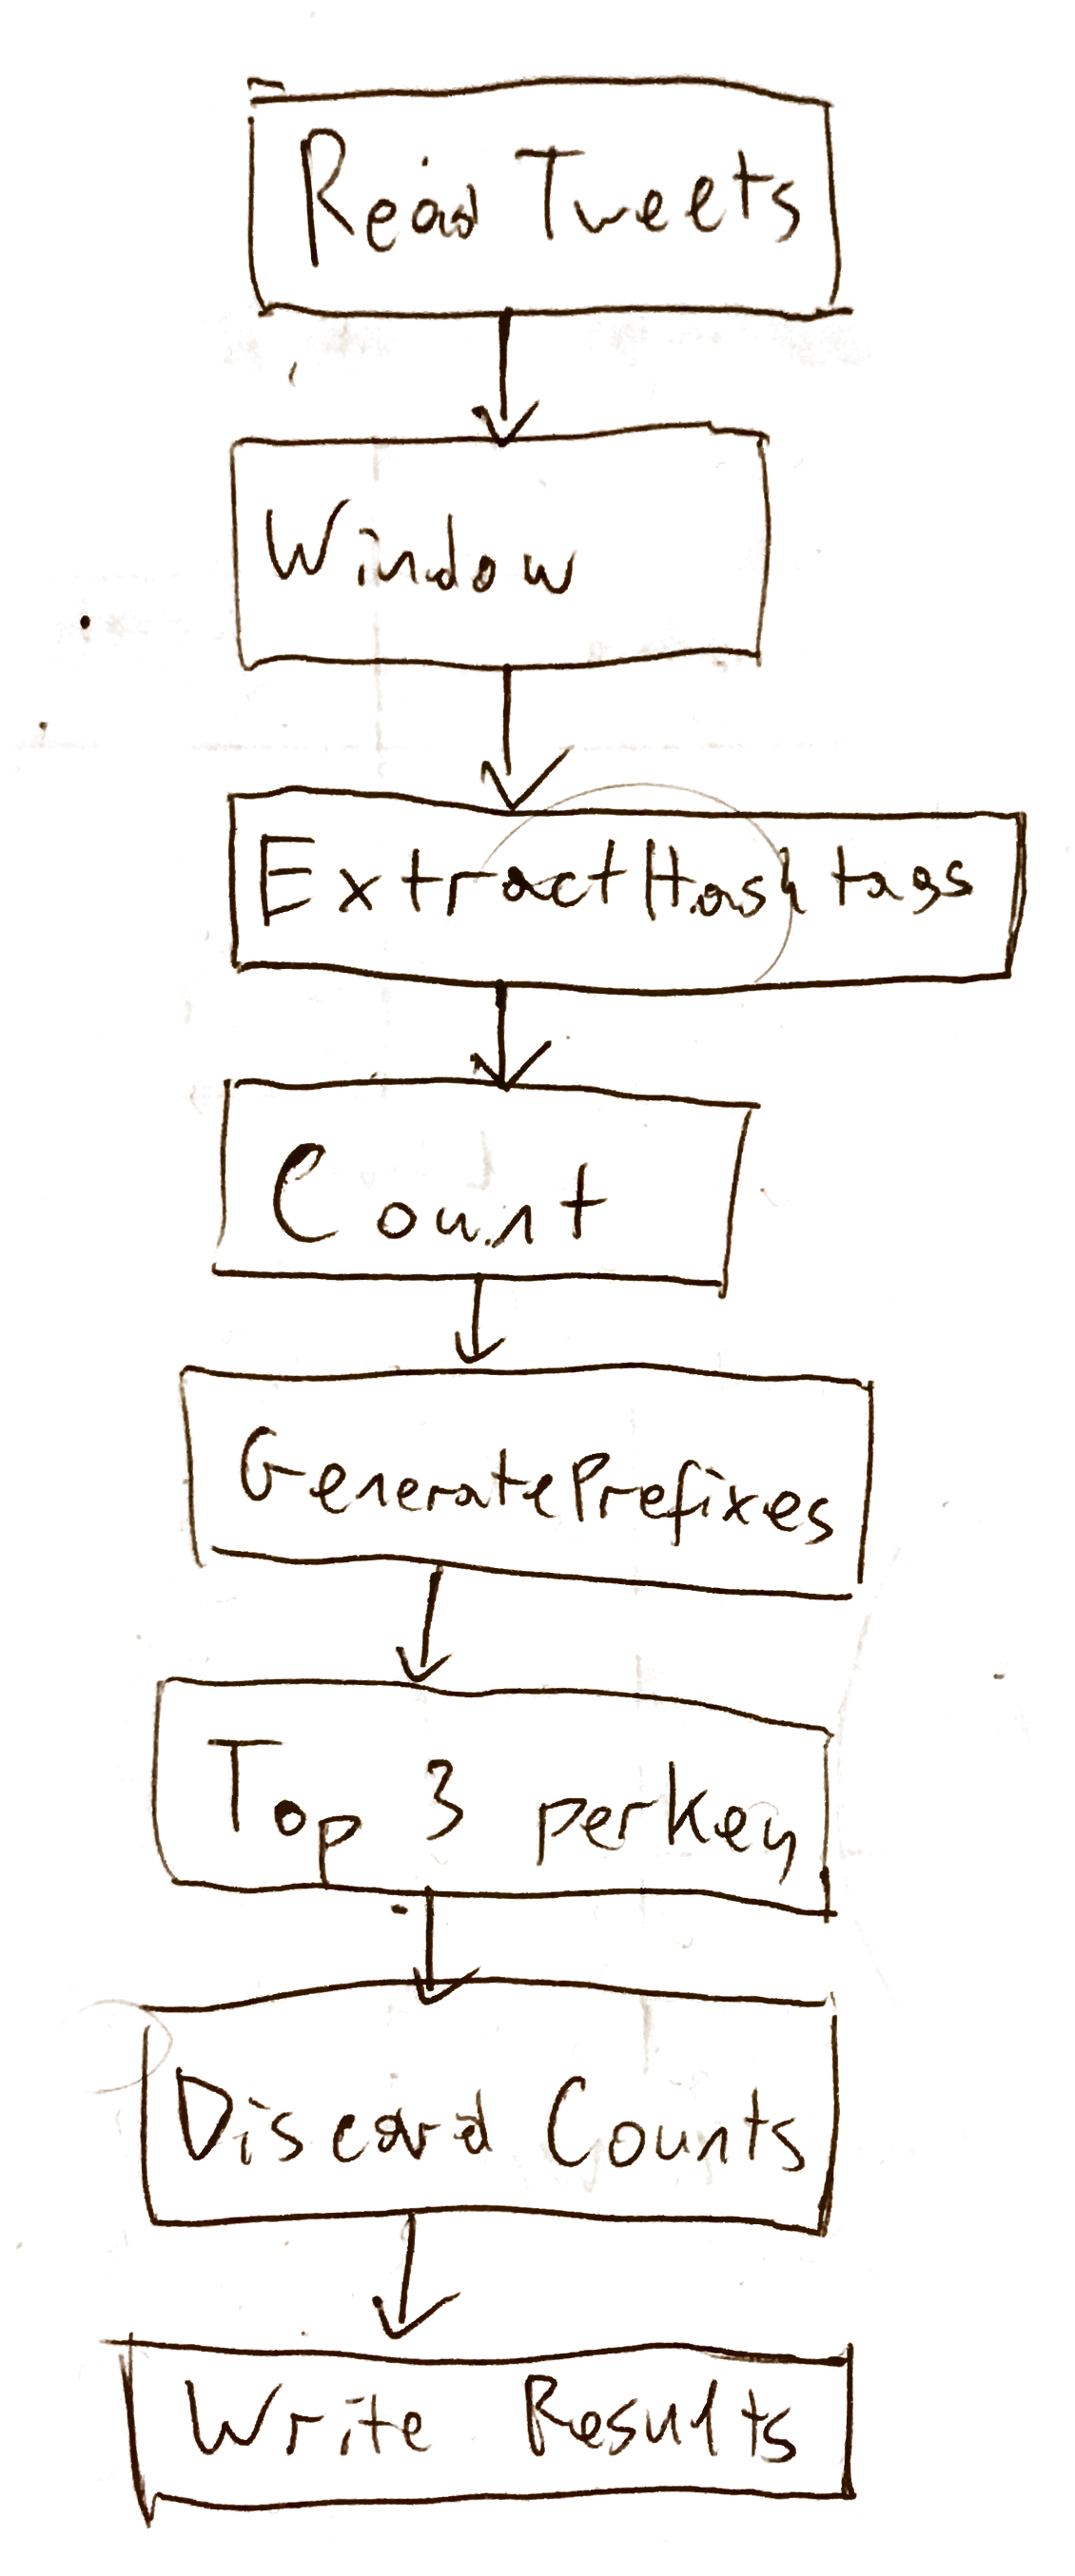
\includegraphics[height=0.5\textheight]{images/temp/eval-twitter-pipeline}
	\caption[The Twitter example Pipeline as a DAG.]{TODO}
	\label{fig:eval:twitter-pipeline-dag}
\end{figure}


The scenario provides a good way to test various features of the Model.
Sliding windowing is used, and multiple stages of aggregation per window is employed.
The Pipeline utilises both Elementwise and Grouping Transforms.

The free stream provided by Twitter delivers only around 100 tweets/second.
Therefore, to exercise the systems and compare their performance under load, both Pipelines included a configurable step which duplicated the tweets by a desired factor, simulating a higher-volume stream.

The key success criterion in this example is not necessarily throughput or latency, due to the bounded amount of input and output per window.
Rather, success is defined as being able to deliver results `on time' for each window.

\subsection{Code comparison}\label{sec:eval:code}

The Pipeline was created in both the Java and Elixir implementations of the Model.
The full code is available in \cref{apx:twitter-code}; what follows is a comparison of selected excerpts which illustrate the differences in the two coding styles.

The Java example is noticeably longer, using XX lines of code (excluding blank lines and comments).
In contrast, the Elixir implementation takes only XX lines of code to write.

\subsubsection{Reading tweets}

One of the primary reasons for the length of the Java version is the required method of injecting the stream of tweets into the Pipeline.

\begin{codelisting}
	\caption{Reading a Twitter stream as an unbounded source in Elixir.}
	\label{lst:eval:twitter-readstream-elixir}
	\begin{minted}[breaklines=true]{elixir}
parse_as_timestamp = fn string ->
  string
  |> Timex.parse!("{WDshort} {Mshort} {0D} {h24}:{0m}:{0s} {Z} {YYYY}")
  |> DateTime.to_unix
  |> DTime.timestamp(:seconds)
end
terms = [...]
#...
p
~> "Read Stream" -- IO.read_stream(fn -> ExTwitter.stream_filter(track: terms, language: "en") end)
~> "Extract Timestamps" -- Windowing.with_timestamps(&parse_as_timestamp.(&1.created_at), delay_watermark: {30, :seconds, :event_time})
# `&parse_as_timestamp.(&1.created_at)` is captured lambda syntax for
# fn tweet -> parse_as_timestamp.(tweet.created_at) end
	\end{minted}
\end{codelisting}

\begin{codelisting}
	\caption[Reading a Twitter stream as an unbounded source in Java.]{Reading a Twitter stream as an unbounded source in Java. Code compressed for readability, the full version (\cref{lst:apxb:twitter-java}) is 194 LoC.}
	\label{lst:eval:twitter-readstream-java}
	\begin{minted}[breaklines=true]{java}
static class DummyCheckpoint
    implements UnboundedSource.CheckpointMark, Serializable { /*...*/ }
    
static class TwitterSource
    extends UnboundedSource<Status, DummyCheckpoint> {
    /*...*/
        
    @Override
    public UnboundedReader<Status> createReader(
        PipelineOptions options,
        @Nullable DummyCheckpoint checkpointMark
    ) throws IOException { /*...*/ }

    protected static class Reader
    extends UnboundedSource.UnboundedReader<Status>
    implements StatusListener {
        /*...*/
        private Reader(String[] terms, TwitterSource source) { /*...*/ }
        @Override public boolean start() throws IOException { /*...*/ }
        @Override public boolean advance() throws IOException { /*...*/ }
        @Override public Status getCurrent() throws NoSuchElementException { /*...*/ }
        @Override public Instant getCurrentTimestamp() throws NoSuchElementException { /*...*/ }
        @Override public void close() throws IOException { /*...*/ }
        @Override public Instant getWatermark() { /*...*/ }
        /*...*/
        @Override public void onStatus(Status status) { /*...*/ }
        /*...*/
    }
}
/*...*/
String[] terms = {/*...*/};

p.apply("GetTweets", Read.from(TwitterSource.withTerms(terms)))
	\end{minted}
\end{codelisting}

The Elixir standard library provides a way to deal with potentially unbounded, lazy data---\exs{Stream}s.
As such, it makes sense that one of the Root Transforms provided out of the box in Elixir Dataflow is \exs{IO.read_stream}.
We need only pass a lambda which creates the desired stream on-demand, and its elements will automatically be emitted.

\Cref{lst:eval:twitter-readstream-elixir} illustrates this well.
\exs{ExTwitter} is a Twiter client for Elixir, and indeed it uses the standard \exs{Stream} module to provide its functionality.

Notable is also the ease with which we can timestamp elements based on their data, and assign them a watermark with a simple, standard Transform.
\exs{Windowing.with_timestamps} is a Composite Transform, so it is easy to insert a smarter watermark heuristic if needed; the one used takes the highest timestamp seen so far and outputs a watermark 30 seconds before this---an element can be up to 30 seconds `out of order' before it is considered late.
This showcases the watermark domains feature (\cref{sec:impl:dataflow:watermark-generation}) not present in the Java implementation.
It is possible to decouple the reading of the stream and the timestamp extraction and watermark generation into separate Transforms, resulting in cleaner, more reusable code.

To achieve the same result in Java, we need almost 200 lines of code, as \cref{lst:eval:twitter-readstream-java} summarises.
Firstly, since there is no standard way of representing streaming sequences in Java, custom source of data will need to implement their own asynchronous logic.
\texttt{Twitter4J}, a popular Twitter client library for Java, requires the user to provide a callback object implementing a particular interface to be notified of new tweets.

In order to `connect' the Twitter stream to the Pipeline, an \texttt{UnboundedSource} had to be written.
This is a large interface requiring the implementation of several functions.
Some of these apply to the advanced distributed features offered by Beam such as checkpointing and coding\footnote{
Used to dump data from memory into storage. In Elixir, no extra coding logic is needed since any term can be serialised in a standard way.
} and are omitted.
Others, however, show the incidental complexity present in the Java API.
On top of this, care must be taken to ensure the class is thread-safe.

Since Beam assumes that the entire Pipeline is in the same watermark domain, the Source itself must manage its own timestamping and watermark generation.
In this case, the class must contain logic not only to read, buffer and emit tweets from the network, but also to extract their timestamp and to generate the delayed watermark based on the data.
This results in long, tightly-coupled and complex code.

Clearly, the conventions around \exs{Stream}s in Elixir coupled with the decoupling of reading and processing logic due to the inclusion of watermark domains are a double-whammy which cause Elixir to come out on top in this comparison.

\subsubsection{Lambdas vs.\ classes}

The Dataflow Model adopts an inherently functional model of computation based on functions transforming data, often using standard patterns of mapping and filtering.
Java's support of this model is poor.
This is exemplified best by the common need to specify logic in small internal classes as in \cref{lst:eval:twitter-lambdas-java}.

\begin{codelisting}
	\caption[Using internal classes to specify transformation logic in Java.]{In Java, there is often a need to use internal classes to specify logic. While Java~8 lambdas can be used, the lack of  type inference means that internal classes are often the cleaner solution.}
	\label{lst:eval:twitter-lambdas-java}
	\begin{minted}[breaklines=true]{java}
 public static class GeneratePrefixesFn
 extends SimpleFunction<KV<String, Long>, List<KV<String, KV<String, Long>>>> {
    @Override
    public List<KV<String, KV<String, Long>>> apply(KV<String, Long> tagWithCount) {
        List<KV<String, KV<String, Long>>> result = new ArrayList<>();
        String downcased = tagWithCount.getKey().toLowerCase();
        for (int i = 1; i <= downcased.length(); i++) {
            String prefix = downcased.substring(0, i);
            result.add(KV.of(prefix, tagWithCount));
        }
     return result;
    }
}
public static class DiscardCountsFn
extends SimpleFunction<KV<String, List<KV<String, Long>>>, KV<String, List<String>>> {
    @Override
    public KV<String, List<String>> apply(KV<String, List<KV<String, Long>>> el) {
        List<String> prefixes = l.getValue().stream().map((KV::getKey)).collect(Collectors.toList());
        return KV.of(el.getKey(), prefixes);
    }
}
/*...*/
.apply("GeneratePrefixes", FlatMapElements.via(new GeneratePrefixesFn()))
/*...*/
.apply("DiscardCounts", MapElements.via(new DiscardCountsFn()))
	\end{minted}
\end{codelisting}

\begin{codelisting}
	\caption[Using lambdas to specify transformation logic in Elixir.]{In Elixir, we take advantage of the inherent functional paradigm of the language to specify transformation logic in a familiar way.}
	\label{lst:eval:twitter-lambdas-elixir}
	\begin{minted}[breaklines=true]{elixir}
~> "Generate Prefixes" -- Core.flat_map(fn {tag, count} ->
  len = String.length tag
  for i <- 0..(len-1), downcased = String.downcase(tag),
    prefix = String.slice(downcased, 0..i),
    do: {prefix, {tag, count}}
 end)
# ...
~> "Discard Exact Counts" -- Core.map(fn {prefix, tcs} ->
  {prefix, Enum.map(tcs, fn {tag, _count} -> tag end)}
 end)
	\end{minted}
\end{codelisting}

\Cref{lst:eval:twitter-lambdas-elixir} shows that Elixir, as a functional language, excels at expressing these kinds of computation natively.

\subsubsection{Summary}

Though formal user studies were not performed to assess the `friendliness' or ease of use of the two SDKs empirically, the preceding examples should show at least that Elixir as a language is much better suited to express the concepts of the Dataflow Model in code.
Java's paradigm is orthogonal to the way computation is reasoned about in the Model, and even though a `fluent API' can be used to make things as friendly as possible, the static typing coupled with no type inference fundamentally limits the expressivity of the language in uses like this one.


\subsection{Performance evaluation}\label{sec:eval:performance}

\subsection{Resource consumption}\label{sec:eval:resource}

\section{Latency evaluation}\label{sec:eval:latency}

A key performance indicator of stream-processing systems is their latency when processing streams of data element-wise.
While much of the power of the Model comes from its grouping and windowing facilities, its goal is to subsume many other models of computation, pure stream processing being one of those.

\subsection{Methodology}

In this experiment, a Pipeline was created in which integer elements were generated in a rate-limited fashion and passed through a series of \verb|Map| Transforms, each of which incremented the element.
The latency of each element from the moment of its generation to its output at the last identity Transform was measured.
The length of the Pipeline was varied and the effects of each on element latency analysed.
CPU and memory usage were also captured at half-second increments.

The experiment was performed with 14 different values for the Pipeline length, ranging from 1 to 2000.
It is to be noted that at length of above approximately 3000 Transforms, the Java implementation fails with a stack overflow, while the Elixir implementation is able to sustain over 10000 Transforms in the Pipeline with the same linear growth.

Each instance of the experiment was repeated X times, each time running for X seconds.
The data from each repetition was aggregated together and a mean and standard deviation calculated.

\subsection{Results}

\todo{Let's discuss the data and how I should frame this.}

\todo{Graphs are of course unstyled and untweaked---they won't look like this.}

\begin{figure}
    \centering
	\subfloat[][As the number of transforms grows, the mean latency increases roughly linearly. (Discuss std dev. \%STDev grows linearly with no transforms.)]{
		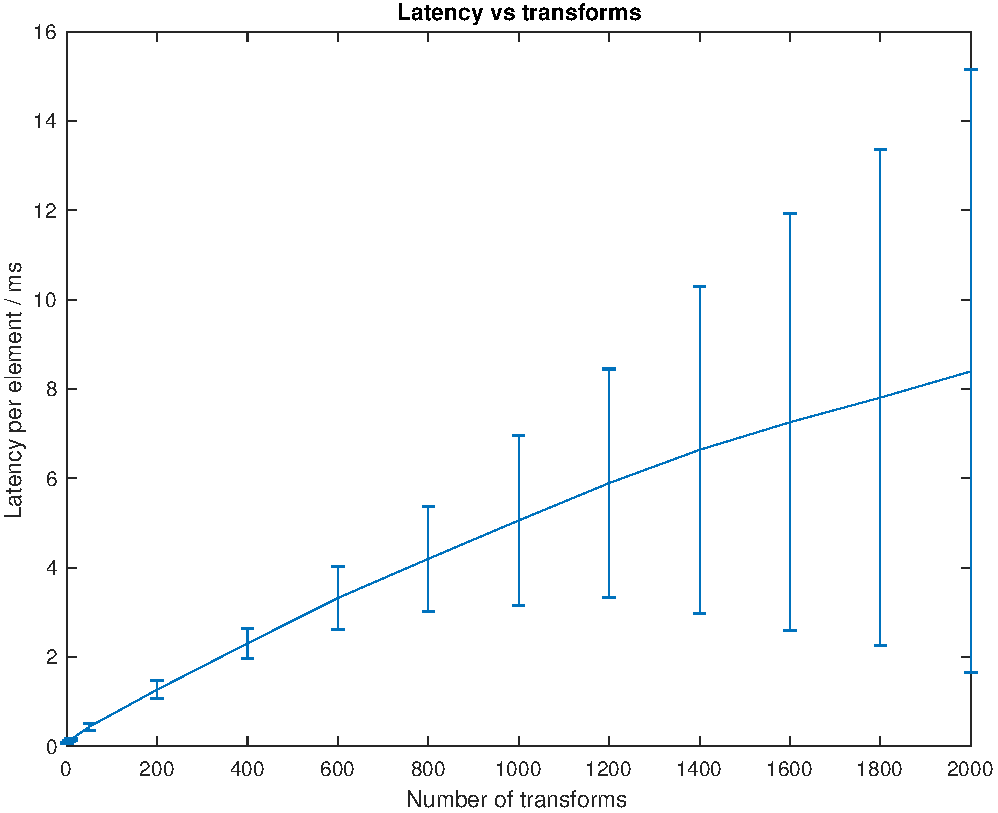
\includegraphics[height=0.45\textheight]{images/temp/elixir_latency}
	}
	
	\subfloat[][]{
		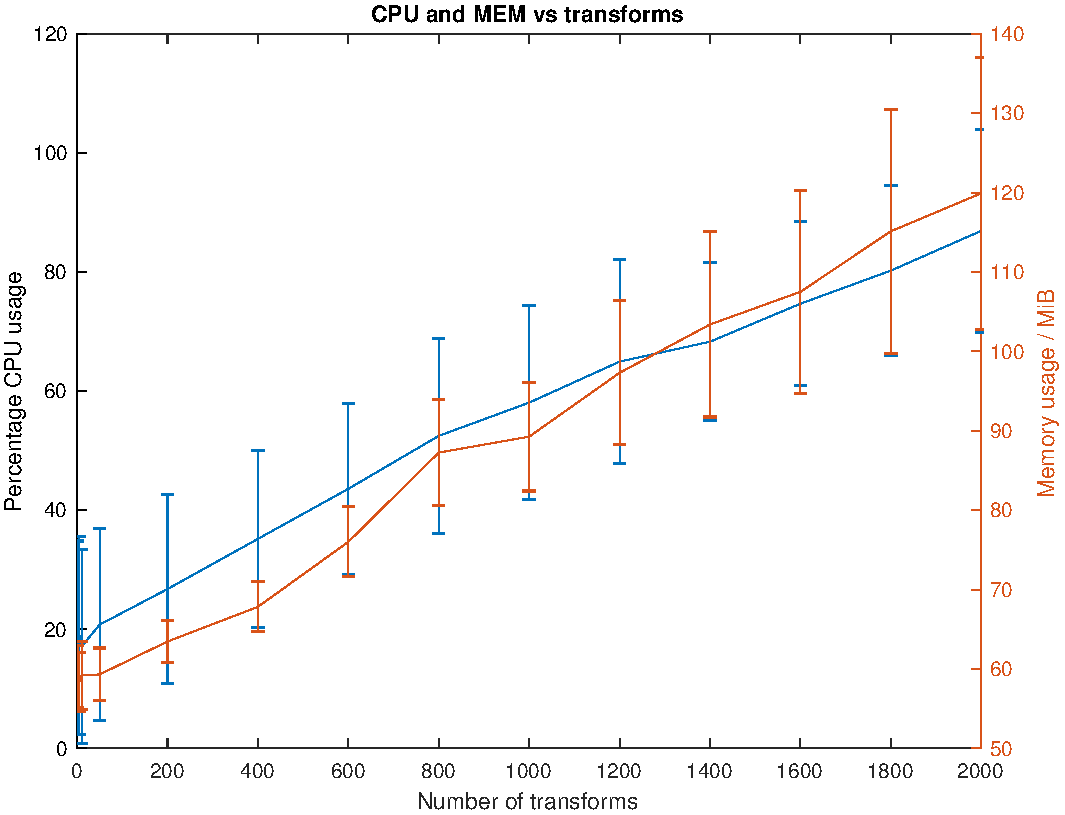
\includegraphics[height=0.45\textheight]{images/temp/elixir_memcpu}
	}
	\caption[Results of the latency experiment run on the Elixir implementation.]{The Elixir implementation shows predictable, linear resource consumption under load.}
	\label{fig:eval:latency-graph-elixir}
\end{figure}

\begin{figure}
    \centering
	\subfloat[][]{
		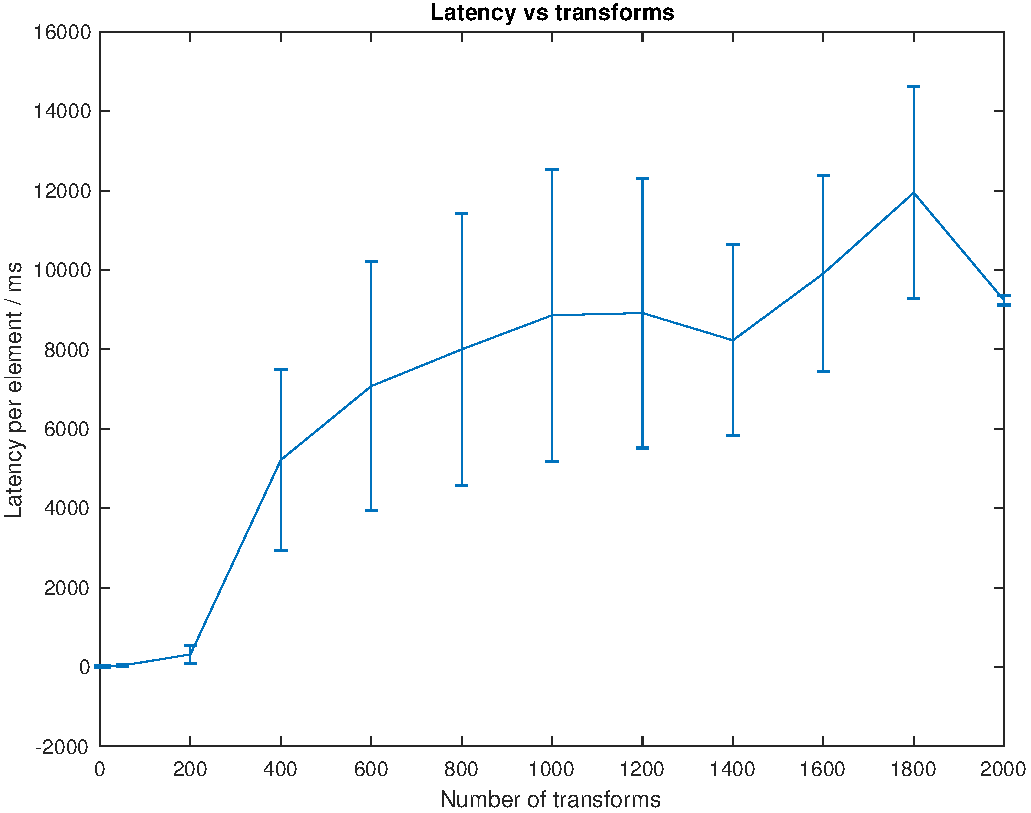
\includegraphics[height=0.45\textheight]{images/temp/java_latency}
	}
	
	\subfloat[][]{
		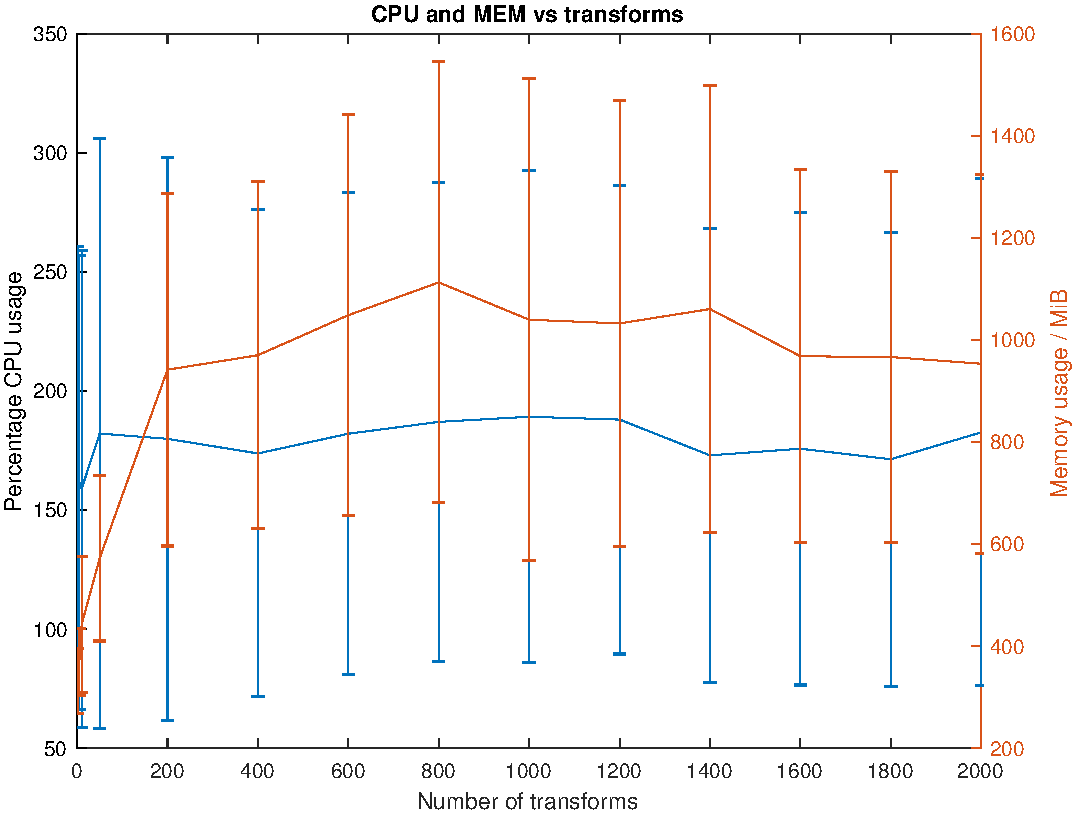
\includegraphics[height=0.45\textheight]{images/temp/java_memcpu}
	}
	\caption[Results of the latency experiment run on the Java implementation.]{The Java implementation shows good behaviour at sub-200 Transform levels, before degrading to very poor levels of latency.}
	\label{fig:eval:latency-graph-java}
\end{figure}
